\documentclass[notitlepage]{nyu22report}
% The `notitlepage' option and the `titling' package provide
% use of the `titlingpage' enviroment. This allows for extra
% text to appear on the title page.
%
% If you have no need for any extra text on the title page,
% you can take out the `notitlepage' option and the `titlingpage'
% environment from the document beginning.
\title{Title of Report}
\subtitle{Subtitle of Report}
\author{Office, unit, or school name}
\date{01/23/2020}

\usepackage{tabularx}% the eponymous environment
\usepackage{threeparttable}% \tnote and \begin{tablenotes}...
\usepackage{colortbl}% color table rows and column backgrounds
\usepackage{enumitem}% customize itemize and enumerate environments
\usepackage{copyrightbox}% the eponymous command
\usepackage{wrapfig}% the wrapfigure environment
\usepackage{lipsum}% lorem ipsum placeholder text

\usepackage{xcolor-nyu22}

\usepackage{fontspec}
\setmainfont[%
    ItalicFont=*,
    ItalicFeatures={FakeSlant},
]{Frank Ruhl Libre}
\setsansfont[%
    ItalicFont=Gotham Book Italic,
    BoldFont=Gotham Medium,
    BoldItalicFont=Gotham Medium Italic,
    FontFace={eb}{\shapedefault}{Gotham Bold},
    FontFace={eb}{it}{Gotham Bold Italic},
    FontFace={l}{\shapedefault}{Gotham Light},
    FontFace={l}{it}{Gotham Light Italic},
]{Gotham Book}
\setmonofont{Inconsolata}

\usepackage{hyperref}
\begin{document}
\begin{titlingpage}
    \maketitle
    Report notes placeholder text
\end{titlingpage}

\tableofcontents

\chapter{Example of Section with Phases}

\section*{Phase 1 (Fall 2020)}
Lorem ipsum dolor sit amet, consectetur adipiscing elit, sed do eiusmod tempor
incididunt ut labore et dolore magna aliqua. Ut enim ad minim veniam, quis
nostrud exercitation ullamco laboris nisi ut aliquip ex ea commodo consequat.

\section*{Phase 2 (Winter 2020)}

Lorem ipsum dolor sit amet, consectetur adipiscing elit, sed do eiusmod tempor
incididunt ut labore et dolore magna aliqua. Ut enim ad minim veniam, quis
nostrud exercitation ullamco laboris nisi ut aliquip ex ea commodo consequat.

\section*{Phase 3 (Spring 2021)}

Lorem ipsum dolor sit amet, consectetur adipiscing elit, sed do eiusmod tempor
incididunt ut labore et dolore mag  na aliqua. Ut enim ad minim veniam, quis
nostrud exercitation ullamco laboris nisi ut aliquip ex ea commodo consequat.


\chapter{Example of Headers and Text Styling}

\section{Header Styles Examples (Heading 3)}

Paragraph (Normal Text). Lorem ipsum dolor sit amet, consectetur adipiscing
elit, sed do eiusmod tempor incididunt ut labore et dolore magna aliqua. A
pellentesque sit amet porttitor eget dolor morbi non arcu.

\subsection{Lorem Ipsum (Heading 4)}

Consectetur libero id faucibus nisl. Sagittis orci a scelerisque purus. Ut sem
viverra aliquet eget sit amet tellus. In massa tempor nec feugiat nisl pretium
fusce id. Facilisi cras fermentum odio eu feugiat pretium nibh.

\subsubsection{Lorem Ipsum (Heading 5)}

Lorem ipsum dolor sit amet, consectetur adipiscing elit, sed do eiusmod tempor
incididunt ut labore et dolore magna aliqua. A pellentesque sit amet porttitor
eget dolor morbi non arcu.

\paragraph{Lorem ipsum (Heading 6)}

Dolor sit amet, consectetur adipiscing elit, sed do eiusmod tempor incididunt ut
labore et dolore magna aliqua. A pellentesque sit amet porttitor eget dolor
morbi non arcu.

\section{Bulleted List Example}

Example of bulleted list:

\begin{itemize}
    \item Bullet list item level one
    \begin{itemize}
        \item Bullet list item level two
        \item Bullet list item level two
        \begin{itemize}
            \item Bullet list item level three
        \end{itemize}
    \end{itemize}
    \item Bullet list item level one
\end{itemize}


\section{Paragraphs Example}

A diam sollicitudin tempor id eu nisl. Turpis in eu mi bibendum neque. Convallis
aenean et tortor at risus. Id faucibus nisl tincidunt eget nullam non nisi.
Tellus in metus vulputate eu scelerisque felis imperdiet.

Faucibus et molestie ac feugiat sed lectus. Augue lacus viverra vitae congue eu
consequat ac felis donec. Integer malesuada nunc vel risus. Egestas maecenas
pharetra convallis posuere morbi leo. Dignissim sodales ut eu sem integer vitae.
Enim sed faucibus turpis in eu mi. Ut sem viverra aliquet eget sit amet tellus
cras adipiscing. In dictum non consectetur a erat nam at lectus.

Sagittis orci a scelerisque purus. Ut sem viverra aliquet eget sit amet tellus.
In massa tempor nec feugiat nisl pretium fusce id. Facilisi cras fermentum odio
eu feugiat pretium nibh. Vitae justo eget magna fermentum iaculis.

Commodo odio aenean sed adipiscing diam donec adipiscing tristique. Quis ipsum
suspendisse ultrices gravida. Nunc sed blandit libero volutpat.

\section{Link Styling Example}

A diam sollicitudin tempor id eu nisl. Turpis in eu mi bibendum neque. Convallis
aenean et tortor \href{https://www.nyu.edu/}{in-line links}. Id faucibus nisl
tincidunt eget nullam non nisi. Tellus in metus vulputate eu scelerisque felis
imperdiet \href{mailto:email@nyu.edu}{email@nyu.edu}. 

\begin{itemize}
    \item Link styling:
    \begin{itemize}
        \item Family: sans serif
        \item weight: bold
        \item underlined
        \item color: primary
    \end{itemize}
\end{itemize}

\chapter{Table Styling}

\begin{threeparttable}
    \newcommand{\theadcellstyle}{\color{white}\bfseries}
    \tabletitle{Chart Title}
    \begin{tabularx}{\textwidth}{|
            >{\bfseries\primarycolor\small}X|
            *2{>{\normalcolor\small}X|}
        }\hline\rowcolor{primary}
        \theadcellstyle Column Header 1
        & \theadcellstyle Column Header 2
        & \theadcellstyle Column Header 3
        \\\hline
        Copy row header text for top row from this cell
        & Copy paragraph styling for top row from this cell
        & \begin{itemize}[left=0pt]
            \item Copy bulleted list styling for top row from this cell
        \end{itemize}
        \\\hline
        Copy row header text for all other rows from this cell
        & Copy paragraph styling for all other rows from this cell
        & \begin{itemize}[left=0pt]
            \item Copy bulleted list styling for all other rows from this cell
        \end{itemize}
        \\\hline
        Lorem ipsum
        & \begin{itemize}[left=0pt]
            \item Lorem ipsum\tnote{*}
        \end{itemize}
        & Lorem ipsum\tnote{**}
        \\\hline
    \end{tabularx}

    \vspace{10pt}
    \begin{tablenotes}\color{MediumGray1}
        \item[*] Chart note text goes here (make sure to add paragraph space before first note)
        \item[**] Chart note text goes here (no paragraph space before second note)
    \end{tablenotes}
\end{threeparttable}

\chapter{Images}

\section*{Image Layout Examples}

This section is meant to give you examples of different image layouts that are
achievable in Google Docs. As a rule of thumb, try to make sure that your images
have ample space around them so that they don’t touch surrounding text. This
gives the page a cleaner look and maintains appropriate legibility.

\subsection*{Single Image}

\copyrightbox[b]
  {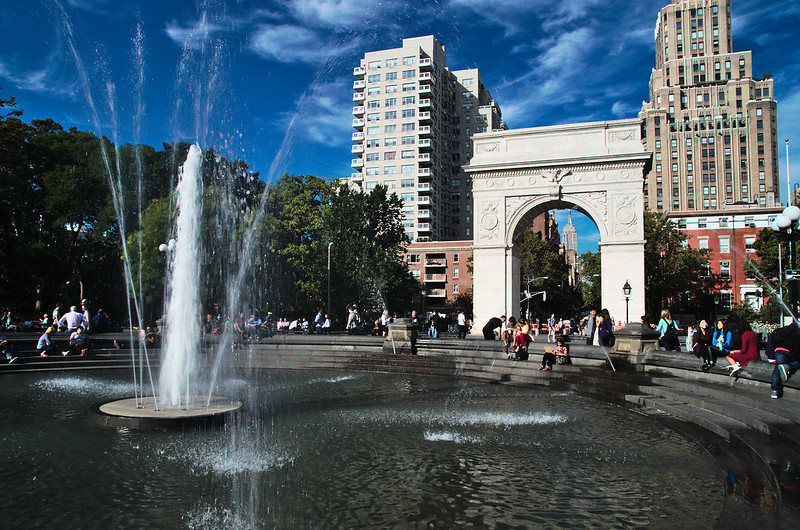
\includegraphics[width=\textwidth]{30812342016_f2cba3be4d_c}}
  {“\href{https://flic.kr/p/eeBz4t}{WashingtonSquarePark}” 
    by \href{https://www.flickr.com/photos/elizaroff/}{himlynx} 
    via Flickr. \href{https://creativecommons.org/licenses/by-nc-nd/2.0/}{CC-BY-NC-ND-2.0}}

\textbf{\primarycolor Quick Tip:} The \texttt{copyrightbox} package makes it
easy to attach a copyright notice to an image. We are using the recommended best
practice for Creative Commons attribution: \textbf{title} (linked to the
source), \textbf{author} (linked to author's page), \textbf{source}, and
\textbf{license} (linked to full text of license).

\subsection*{Two Images (50/50)}

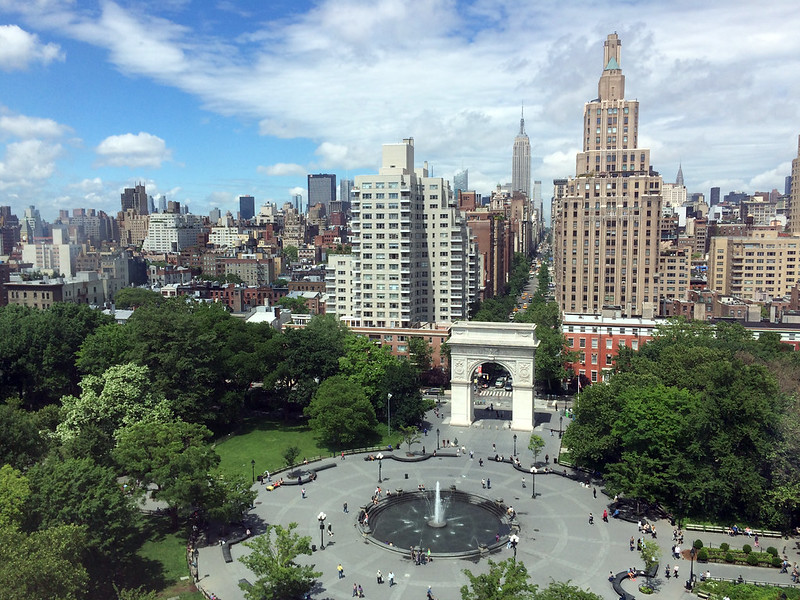
\includegraphics[width=0.495\textwidth]{14168452957_bf270cd3bd_c}
\hfill
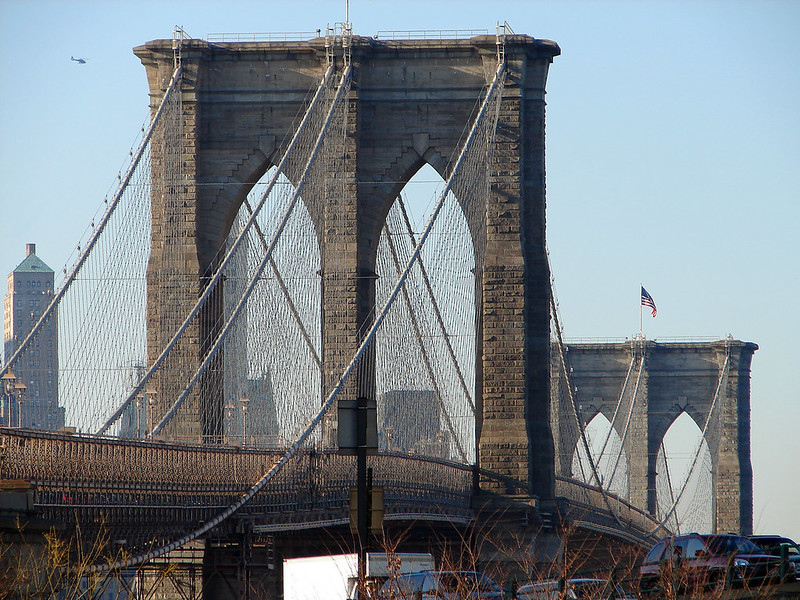
\includegraphics[width=0.495\textwidth]{5809293214_756213372f_c}

\textbf{\primarycolor Quick Tip:}
It is also allowable to attribute Creative Commons licensed images at the end of
the document, as we have done below.


\section*{Single Image, Left-wrapped Text}

\begin{wrapfigure}{r}{0.5\textwidth}
    \begin{center}
      
\includegraphics[width=0.48\textwidth]{14116552080_90958b7fc9_c}
    \end{center}
  \end{wrapfigure}
Wrapping text around images is harder in \LaTeX{} than in Microsoft Word or
Google Docs, but it can be accomplished with the \texttt{wrapfig} package and the
\texttt{wrapfigure} enviroment. Things can get complicated when the surrounding
text is shorter than the vertical height of the wrapped image, and list
environments such as \texttt{itemize} are used.

\lipsum[1]

\subsection*{Single Image, Right-wrapped Text}

\begin{wrapfigure}{l}{0.5\textwidth}
    \begin{center}
      
\includegraphics[width=0.48\textwidth]{8321394957_a70473000d_c}
    \end{center}
  \end{wrapfigure}
If you want your image on the left hand side of your text, use the \texttt{l}
argument for the \texttt{wrapfigure} enviroment. 

\lipsum[2]

\subsection*{Image Descriptions and Accessibility}

Images add great value to the web browsing experience, and can be a very
accessible way of conveying information. But, unless a text equivalent is
provided, information in images cannot be accessed or understood by users who
cannot see them. This can result in screen reader users not being able to
understand content or understand how to interact with content.

Adding alt text to images in PDFs is not as easy as it is with HTML. There are
some \LaTeX{} packages in development but the project is far from complete. Read
more about image descriptions on NYU’s
\href{https://www.nyu.edu/life/information-technology/help-and-service-status/accessibility/accessibility-checklist/image-descriptions-text-alternative.html}{Digital
Accessibility Checklist}.

\appendix
\chapter{Image attributions}

\begin{itemize}
    \item “\href{https://flic.kr/p/eeBz4t}{WashingtonSquarePark}” 
    by \href{https://www.flickr.com/photos/elizaroff/}{himlynx} 
    via Flickr. \href{https://creativecommons.org/licenses/by-nc-nd/2.0/}{CC-BY-NC-ND-2.0}
    \item \href{https://flic.kr/p/nA22rF}{2014\_06\_05\_nyc-from-nyu\_16}
    by \href{https://www.flickr.com/photos/docsearls/}{Doc Searls}
    via Flickr.
    \href{https://creativecommons.org/licenses/by/2.0/}{CC-BY-2.0}
    \item “\href{https://flic.kr/p/9Rm9tQ}{Brooklyn Bridge}”
    by \href{https://www.flickr.com/photos/3336/}{Diego Torres Silvestre}
    via Flickr.
    \href{https://creativecommons.org/licenses/by/2.0/}{CC-BY-2.0}
    \item “\href{https://flic.kr/p/nvr27Y}{All Day, All Night, NYU}” by \href{https://www.flickr.com/photos/wwward0/}{Billie Grace Ward} via Flickr.
    \href{https://creativecommons.org/licenses/by/2.0/}{CC-BY-2.0}
    \item “\href{https://flic.kr/p/dFkjNR}{New York University}” 
       by \href{http://scottbeale.org/}{Scott Beale} via Flickr.
    \href{https://creativecommons.org/licenses/by-nc-nd/2.0/}{CC-BY-NC-ND-2.0}
\end{itemize}

\end{document}
